\documentclass[../solutions_manual.tex]{subfiles}
\begin{document}
\ifSubfilesClassLoaded{\setcounter{chapter}{10}}{}% NN-1 when built standalone
\setcounter{chapter}{10}% NN-1, so this chapter is numbered NN
\chapter{The $\Psi$ Ratio: Measuring Formation}\label{sol11}
\sloppy

All numbers below are printed by \texttt{python3} \nolinkurl{code/solutions/sol11.py}. Variances of fixed effects are population variances (divisor $n$), as in \texttt{code/ch11.py}. Throughout, $\hat\Psi_{\text{var}}$ is the descriptive variance ratio of Definition~\ref{ch11:thm:cohort_year}, \emph{not} the $\Psi$ of Definition~\ref{ch09:def:psi}.

%% ---------------------------------------------------------------------
\exercisesolution{11.1}{Cohort--year decomposition by hand}
The grand mean of the nine cells is $0.5389$.

\solpart{a} Year means (average over cohorts) are $0.4933$ (1980), $0.5433$ (1990) and $0.5800$ (2000). Centred, the year effects are $\hat\alpha_t = (-0.0456, 0.0044, 0.0411)$.

\solpart{b} Cohort means minus the grand mean give $\hat\delta_c = (-0.1256, 0.0044, 0.1211)$ for the 1940s, 1950s and 1960s cohorts. In a balanced table these row and column means are the OLS estimates of the two-way model~\eqref{ch11:eq:cohort_year} (with no covariates). The residuals are small but not zero; the largest are $0.0189$ and $-0.0144$, in the corners, so the additive model does not fit exactly. That curvature is what an age profile would pick up.

\solpart{c} $\Var(\hat\alpha_t) = 0.001262$ and $\Var(\hat\delta_c) = 0.010151$, so
\[
\hat\Psi_{\text{var}} = \frac{0.010151}{0.001262} = 8.045 .
\]

\solpart{d} Under the two-way specification (no age effects), cohort effects are far more dispersed than year effects: their standard deviation is $\sqrt{8.045} = 2.8$ times larger. But see (e).

\solpart{e} Ages (cohort mid-years 1945, 1955, 1965) are:
\begin{center}
\begin{tabular}{lccc}
\toprule
& 1980 & 1990 & 2000 \\
\midrule
Born 1940s & 35 & 45 & 55 \\
Born 1950s & 25 & 35 & 45 \\
Born 1960s & 15 & 25 & 35 \\
\bottomrule
\end{tabular}
\end{center}
Index cohorts and years by decade, $c, t \in \{0, 1, 2\}$, so the age index is $a = t - c$. By Proposition~\ref{ch11:prop:apc}, $(\hat\alpha_t - kt,\ \hat\delta_c + kc,\ A_a = ka)$ gives fitted values identical to the two-way fit for every $k$; the script checks this cell by cell. The variance ratios are:
\begin{center}
\begin{tabular}{lccc}
\toprule
$k$ (per decade) & cohort effects $\hat\delta_c + kc$ & year effects $\hat\alpha_t - kt$ & $\hat\Psi_{\text{var}}$ \\
\midrule
$-0.10$ & $(-0.026, 0.004, 0.021)$ & $(-0.146, 0.004, 0.141)$ & 0.027 \\
$-0.05$ & $(-0.076, 0.004, 0.071)$ & $(-0.096, 0.004, 0.091)$ & 0.618 \\
$0$ & $(-0.126, 0.004, 0.121)$ & $(-0.046, 0.004, 0.041)$ & 8.045 \\
$+0.05$ & $(-0.176, 0.004, 0.171)$ & $(0.004, 0.004, -0.009)$ & 507.250 \\
\bottomrule
\end{tabular}

{\small Effects centred to mean zero.}
\end{center}
Since $\Var(c) = \Var(t)$, the $k^2$ terms cancel in $\Var(\hat\delta_c + kc) - \Var(\hat\alpha_t - kt)$. The ratio therefore equals one at a single value,
\[
k^* = \frac{\Var(\hat\alpha) - \Var(\hat\delta)}{2\,[\Cov(\hat\delta, c) + \Cov(\hat\alpha, t)]} = \frac{0.001262 - 0.010151}{2\,(0.08222 + 0.02889)} = -0.0400 .
\]
The extremes of Proposition~\ref{ch11:prop:apc} are reached at the least-squares slopes. At $k_\delta = -0.1233$, which detrends the nearly linear cohort effects, $\hat\Psi_{\text{var}} = 0.0005$. At $k_\alpha = 0.0433$, which detrends the year effects, it is $1876$. As $|k| \to \infty$ the ratio tends to $\Var(c)/\Var(t) = 1$.

\textit{What (d) depends on.} The answer depends entirely on the unidentified linear trend $k$, i.e.\ on the APC restriction. Reporting ``cohort effects dominate'' means choosing $k > -0.04$; reporting ``year effects dominate'' means choosing $k < -0.04$. The data identify only the \emph{curvature} (second differences) of the three sets of effects. Here each set has only three points, so a single second difference each. \textit{Common mistake:} treating the two-way fit without age effects as neutral. Omitting age effects is itself a restriction ($A_a \equiv 0$), and it loads the life-cycle profile onto cohorts and years.

%% ---------------------------------------------------------------------
\exercisesolution{11.2}{Epidemiological design}
\solpart{a} For daughter $i$ of parents from origin $A \in \{A, \ldots, J\}$, living in Argentina (Definition~\ref{ch11:def:epi}):
\[
\text{LFP}_{i} = \alpha + \beta\,\text{LFP}_{A(i),t_0} + \gamma'Z_i + \varepsilon_i ,
\]
where $\text{LFP}_i \in \{0,1\}$ and $\text{LFP}_{A,t_0}$ is origin female LFP around the parents' emigration. $Z_i$ contains age, survey year and region of residence. It should \emph{not} include the daughter's education, marital status or fertility, which are bad controls (Proposition~\ref{ch11:thm:epi_id}, caveats). Parental education is a separate case: it is a pre-determined control. The regressor varies only across ten origins, so standard errors must be clustered by origin. With ten clusters, use a wild-cluster bootstrap.

\solpart{b} $\hat\beta = 0.35$: a daughter whose parents come from a country with 10~pp higher female LFP is $3.5$~pp more likely to participate, facing the same Argentine labour market. Across the full range of origins (0.20 to 0.75) the predicted difference is $0.35\times 0.55 = 0.1925$, i.e.\ 19~pp. Under Proposition~\ref{ch11:thm:epi_id}, $\beta = \rho\lambda$ with reliability $\lambda \in [0,1]$, so $0.35$ is a \emph{lower bound} on the per-generation persistence $\rho$. It is not $\rho$ itself, because origin LFP also contains origin enforcement ($e_A$).

\solpart{c} Ten evenly spaced origin rates from 0.20 to 0.75 have spacing $0.0611$ and population variance $\Var(\text{LFP}_A) = 0.0611^2\,(10^2 - 1)/12 = 0.030810$. The variance explained by origin is $\hat\beta^2\Var(\text{LFP}_A) = 0.1225\times 0.030810 = 0.003774$. Hence
\[
\text{share explained} = \frac{0.003774}{0.003774 + 0.04} = 8.6\% .
\]
(With the $n-1$ divisor the variance is $0.034234$ and the share $9.5\%$.) This is not $\Psi$, for three reasons.
\begin{itemize}
\item $\Psi$ is a ratio of the formation effect to the enforcement effect of \emph{one perturbation} (Definition~\ref{ch09:def:psi}). The $R^2$ share is a ratio of variances in a cross-section.
\item With a single host country, there is no enforcement variation in the regression at all. The residual variance $0.04$ is individual heterogeneity, not enforcement (Appendix~\ref{ch11:app:epi}).
\item A small explained share is fully compatible with a large $\Psi$ for a given policy, and vice versa.
\end{itemize}

\solpart{d} Generalize assumption~2 of Proposition~\ref{ch11:thm:epi_id} to $\theta_m = \theta_A + \sigma_A$, where $\sigma_A$ is the selection of migrants on $\theta$ relative to their origin, and let the daughter's residual $u_d$ possibly correlate with origin. Repeating the proof,
\[
\beta = \frac{\Cov(\text{LFP}_d, \text{LFP}_A)}{\Var(\text{LFP}_A)} = \rho\lambda + \frac{\rho b\,\Cov(\sigma_A, \text{LFP}_A) + \Cov(u_d, \text{LFP}_A)}{\Var(\text{LFP}_A)} .
\]
Selection inflates $\hat\beta$ (given $b, \rho > 0$) when either term is positive.
\begin{itemize}
\item $\Cov(\sigma_A, \text{LFP}_A) > 0$: emigrants from high-LFP origins are \emph{more} work-oriented than their origin average, relative to emigrants from low-LFP origins. Equivalently, selection on $\theta$ differs by origin in the same direction as origin culture.
\item $\Cov(u_d, \text{LFP}_A) > 0$: migrants from high-LFP origins bring more of something else that raises daughters' work, such as parental education, wealth, or ethnic job networks in Argentina.
\end{itemize}
Uniform selection (the same $\sigma_A$ for every origin) does not bias $\beta$; it is absorbed in the constant. \textit{Remedies:} control for parental education and occupation; compare origins with similar emigrant selection; use third generations (the ratio $\beta_3/\beta_2 = \rho$ removes $\lambda$, though not differential selection).

%% ---------------------------------------------------------------------
\exercisesolution{11.3}{What adoption designs can and cannot tell you}
\solpart{a} The design randomizes adoptees across \emph{adoptive} families, so it identifies the effect of the adoptive family's environment. The adoptees' biological parents (in Korea) are not observed in the data, and their characteristics do not vary in a way the design controls. Even if they were observed, their effect would bundle genes with the prenatal and pre-adoption environment. The design therefore has no variation that isolates the biological parents. What it delivers is the contrast between the adoptive-mother gradient for adoptees (environment) and the gradient for biological children (environment plus genes).

\solpart{b} Under the additive model, gradient $=$ environment $+$ genes. The adoptee gradient $0.10$ estimates the environment component, and $0.30 - 0.10 = 0.20$ the genetic component. The environment share of the biological-child gradient is $0.10/0.30 = 1/3$. Two caveats: additivity rules out gene--environment interaction, and adoptees may respond differently to the same environment (age at adoption, discrimination).

\solpart{c} Let schooling be $S = a + b\theta + u$ for both mother and child, with $u$ independent of $\theta$ and across generations. Let transmission be environmental only, $\theta_{\text{child}} = \rho\theta_{\text{mother}} + \text{const} + \text{noise}$, as in Proposition~\ref{ch11:prop:id_params}(1). Then the adoptee gradient is
\[
\frac{\Cov(S_{\text{child}}, S_{\text{mother}})}{\Var(S_{\text{mother}})} = \rho\,\frac{b^2\Var(\theta)}{\Var(S)} = \rho R_\theta .
\]
So $0.10 = \rho R_\theta$, and $\rho = 0.10/R_\theta \ge 0.10$. With $R_\theta = 1$, $0.5$ or $0.25$, the implied $\rho$ is $0.10$, $0.20$ or $0.40$. The additional assumptions needed are:
\begin{itemize}
\item the share $R_\theta$ of schooling variance due to $\theta$ (or $b$ and $\Var\theta$);
\item that the mapping $S = a + b\theta + u$ is linear and the same across generations;
\item that the mother's schooling affects the child \emph{only} through $\theta$, and not through income or resources. Otherwise the gradient overstates $\rho$.
\end{itemize}

\solpart{d} Yes, it is consistent, but only for the \emph{non-shared} part of $W^I$. ``Common family environment'' in a twin design is everything twins raised together share. That includes much non-family $W^I$: the same neighbourhood, often the same school, the same local media. So little common-environment variance in risk attitudes \citep{cesarini2009genetic} also limits formation through shared peers and media. It leaves room for formation through individual-specific links (one's own friends, workplace) and own experience, the diagonal of $W^I$ (Stylized Fact~\ref{ch11:prop:risk}). \textit{A test.} Randomly assigned college roommates, following the design of \citet{sacerdote2001peer}:
\begin{itemize}
\item \emph{Treatment:} the baseline risk attitude of one's randomly assigned roommate, elicited with an incentivized lottery task before assignment.
\item \emph{Outcome:} one's own risk attitude after one year, with own baseline and dorm fixed effects as controls.
\item \emph{Identification:} institutional random assignment removes homophily (item 3 of Section~\ref{ch11:sec:network}). Using pre-assignment roommate traits avoids the reflection problem. Dorm fixed effects absorb common shocks.
\item \emph{Power:} for an effect of $0.10$~SD per SD of roommate risk tolerance, with residual SD $0.8$, $\alpha = 0.05$ (two-sided) and power $0.80$: $n = [(1.960 + 0.842)\times 0.8/0.10]^2 = 502.3$, i.e.\ 503 students. Without the baseline control (residual SD $1.0$) the requirement is 785; for a $0.05$~SD effect it is 2010. Pairs share shocks, so cluster by room; the requirement then rises by the design effect.
\end{itemize}
A positive coefficient is a formation effect of a specific $\Delta W^I$, which is what Definition~\ref{ch09:def:psi} asks for.

%% ---------------------------------------------------------------------
\exercisesolution{11.4}{Bolivia's self-employment variance ratio}
\textbf{Data status.} The \textit{Encuesta de Hogares} microdata are \emph{not} in \texttt{data/processed}. They are on INE's ANDA portal and were not fetched (\texttt{data/README.md}, \S9). The cohort--year results below are therefore method only; no cohort or departmental value is reported. The one real input available is the \emph{national} self-employment share by survey year, from ILOSTAT (dataflow \nolinkurl{DF_EMP_TEMP_SEX_STE_NB}, retrieved 2026-11-05; file \nolinkurl{data/processed/ilostat_bolivia_emp_status.csv}). Self-employed (\nolinkurl{STE_AGGREGATE_SLF}: employers, own-account and contributing family workers) over total employment, both sexes:
\begin{center}
\footnotesize\setlength{\tabcolsep}{3.5pt}
\begin{tabular}{lcccccccccc}
\toprule
year & 2000 & 2002 & 2003$^\dagger$ & 2005 & 2007 & 2009$^\dagger$ & 2013$^\dagger$ & 2015$^\dagger$ & 2016 & 2019 \\
\midrule
self-employed, \% & 68.4 & 68.5 & 64.0 & 66.0 & 62.7 & 58.2 & 60.9 & 61.6 & 70.0 & 66.6 \\
\bottomrule
\end{tabular}
\end{center}
$^\dagger$ ILOSTAT source ``HIES -- Household Survey''; the other years are ``LFS -- Encuesta Continua de Empleo''. Over the 19 survey years 2000--2019 (none in 2010) the mean is $64.6\%$, the range $58.2\%$ (2009) to $70.0\%$ (2016), and the SD of the yearly shares $3.52$~pp. The LFS years average $67.1\%$ and the HIES years $61.2\%$, which suggests a survey-type break. The year effects must therefore include survey-instrument dummies, or else instrument changes are read as ``labour-market conditions''. The WDI modelled 2019 value is $68.1\%$.

\solpart{a} \emph{Cells.} Pool the EH rounds 2000--2019 (omitting 2010, when there was no survey). Keep employed persons aged 15--64 and define self-employment as above (or own-account only, as a robustness check). Assign five-year birth cohorts, 1935--39 to 1995--99. Compute weighted cell means $\bar x_{c,t}$ using the expansion factors, together with cell sizes and sampling variances, and drop cells with fewer than about 100 observations. Restrict to ages 25--64 for the main specification, so that schooling exit does not drive the youngest cells.

\solpart{b} \emph{Estimation.} Regress $\bar x_{c,t}$ by WLS (weights $=$ inverse sampling variance) on year dummies, cohort dummies, and composition controls (education shares, urban share, sector shares by cell). Year dummies capture labour-market conditions and survey-instrument changes; cohort dummies capture norm persistence. An alternative is to estimate at the individual level with the same dummies and cluster by cohort $\times$ year.

\solpart{c} \emph{Restriction and sensitivity.} Self-employment has a strong life-cycle profile, so age effects cannot be omitted, and one linear restriction is needed (Proposition~\ref{ch11:prop:apc}).
\begin{itemize}
\item \emph{Main specification:} Deaton's normalization (year effects orthogonal to a linear trend and summing to zero; \citealt[\S2.7]{deaton1997analysis}).
\item \emph{Alternative:} equal effects for the two oldest cohorts, or an external age profile (for example from a single cross-section, with year effects set to zero for that year).
\end{itemize}
Report $\hat\Psi_{\text{var}}$ under both and the whole curve $\hat\Psi_{\text{var}}(k)$, as in Exercise~11.1. Bias-correct both variances by subtracting the mean sampling variance of the estimated effects (Appendix~\ref{ch11:app:cohort_year}), and F-test $\delta_c = 0$. \emph{Expected qualitative result} (not an estimate): Deaton's normalization assigns all trends to age and cohort, so it tends to produce a large $\hat\Psi_{\text{var}}$. The national year shares above move by only a few points, apart from the survey-type break. The ranking of cohort vs.\ year dispersion is likely to reverse under alternative restrictions, as in Exercise~11.1.

\solpart{d} Repeat (a)--(c) separately for La Paz (urban) and the rural Altiplano, defined from the department and urban/rural identifiers (rural La Paz, Oruro and Potosí). The comparison \emph{cannot} by itself show that formation is stronger where $W^I$ is more block-diagonal.
\begin{enumerate}
\item $\hat\Psi_{\text{var}}$ is a ratio: a higher value in one region may reflect smaller year-effect variance (more stable local labour demand), not more cohort dispersion.
\item Rural self-employment is mostly own-account farming. Its persistence across cohorts reflects land tenure and the absence of wage jobs, which is enforcement, not norms.
\item Internal migration (Altiplano to El Alto and La Paz) changes the composition of regional cohorts over time. Selective out-migration creates spurious cohort effects.
\item The APC restriction may be valid in one region and not in the other.
\end{enumerate}
One would need: a measure of $W^I$ by region (network modules in the EH, or proxies such as language, media access and migration ties); an internal epidemiological design (migrants from high- vs.\ low-self-employment departments now in the same city; Example~\ref{ch11:prop:bolivia}(3)); and ideally variation in exposure that is plausibly exogenous, such as rollout of roads, radio or mobile coverage.

%% ---------------------------------------------------------------------
\exercisesolution{11.5}{The WWII natural experiment}
\textbf{Data status.} The figures ($\sim$28\%, $\sim$36\%, $\sim$33\%) are the exercise's illustrative values. The Census/BLS series were not fetched (\texttt{data/README.md}, row 22), so no other value is used.

\solpart{a} Two observations cannot separate two effects plus a trend without assumptions, so we state them. (i) The wartime rise $28 \to 36$ (8~pp) is enforcement: mobilization raised labour demand at fixed preferences. (ii) Demobilization removed that demand by 1950. (iii) There is no pre-war secular trend. Under (i)--(iii), the 1950 level decomposes as
\[
\underbrace{33 - 28}_{5\text{ pp}} = \underbrace{E_{1950}}_{\approx 0} + \underbrace{F_{1950} + \text{persistence among wartime workers}}_{5\text{ pp}} .
\]
If instead LFP had a pre-war trend of $\tau$~pp per year, the residual is $5 - 10\tau$: $3$~pp at $\tau = 0.2$, $2$ at $0.3$, $0$ at $0.5$. The ``formation'' share is therefore only as good as the counterfactual trend.

\solpart{b} Yes, partly. Between 1945 and 1950 LFP fell by 3~pp, i.e.\ $37.5\%$ of the 8~pp wartime gain was reversed and $62.5\%$ was not. Under (ii), all of the reversal is the enforcement effect switching off. That enforcement reverses is consistent with the evidence the book cites that much of the wartime entry was reversed by 1950 \citep{goldin1991role}.

\solpart{c} The 5~pp that persisted cannot be cross-generational formation yet. Daughters of wartime workers were mostly children in 1950. Formation through them (Chapter~9: preferences formed in childhood through $W^I$) would show up as \emph{cohort} effects for women born roughly 1930--1945, as they entered the labour market in the 1950s and 1960s. The 1950 persistence comes instead from the wartime cohorts themselves. That can be own-experience formation (the diagonal of $W^I$, as in Stylized Fact~\ref{ch11:prop:risk}), or human capital and job attachment acquired during the war. The latter is state dependence at fixed preferences, i.e.\ enforcement. A related cross-generational channel runs through sons: men whose mothers worked are more likely to have working wives \citep{fernandez2004mothers}. The test is a cohort comparison in later censuses: do women who were children in high-mobilization states work more as adults, after year and age effects?

\solpart{d} Definition~\ref{ch09:def:psi} needs a \emph{permanent} perturbation, an outcome, an agent group and a horizon. The war was a \emph{temporary} $\Delta W^P$ (1941--45). Measured after it ended, its enforcement effect is $E \approx 0$, so a $\Psi$ for ``the war'' is undefined or meaningless. Well-posed alternatives:
\begin{itemize}
\item The perturbation is the permanent $\Delta W^I$ the war left behind (daughters' exposure to working mothers and to women in market jobs); the outcome is daughters' adult LFP; the horizon is one generation. A pure $\Delta W^I$ has $E = 0$ (Proposition~\ref{ch10:prop:levers}(3)), so again one reports $F$, not $\Psi$.
\item The perturbation is a permanent rise in female labour demand (a $\Delta W^P$ that stays), with outcome women's LFP and horizon $T = 1, 2$ generations. Then $E > 0$ persists and $\Psi(\Delta W^P, T) = F/E$ is defined.
\end{itemize}
The war is the temporary version of the second case. It identifies hysteresis (persistence after the shock is removed), which in the affine formation model can come only from a lasting change in $W^I$ or in human capital. A transient $\Delta W^P$ with an unchanged $W^I$ decays at rate $\rho$ (Proposition~\ref{ch09:thm:hysteresis}).

%% ---------------------------------------------------------------------
\exercisesolution{11.6}{Sensitivity analysis}
With $\kappa = \mu\beta\eta$ and $\lambda = \rho + \kappa$, Proposition~\ref{ch10:prop:psi_lq} gives $\Psi(\infty) = \kappa/(1 - \lambda)$. At $\mu = 0.18$, $\beta\eta = 0.5$, $\kappa = 0.09$.

\solpart{a} Varying $\rho$ (at $\mu = 0.18$):
\begin{center}
\begin{tabular}{lcccc}
\toprule
$\rho$ & 0.50 & 0.62 & 0.75 & 0.90 \\
\midrule
$\Psi(\infty)$ & 0.220 & 0.310 & 0.562 & 9.000 \\
\bottomrule
\end{tabular}
\end{center}
\begin{center}
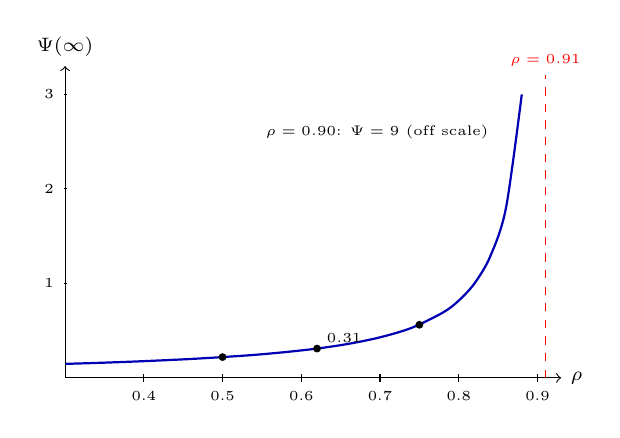
\begin{tikzpicture}[xscale=10, yscale=1.2]
\draw[->] (0.30,0) -- (0.93,0) node[right, font=\scriptsize] {$\rho$};
\draw[->] (0.30,0) -- (0.30,3.3) node[above, font=\scriptsize] {$\Psi(\infty)$};
\foreach \r in {0.4,0.5,0.6,0.7,0.8,0.9} {\draw (\r,0.04) -- (\r,-0.04) node[below, font=\tiny] {\r};}
\foreach \y in {1,2,3} {\draw (0.302,\y) -- (0.298,\y) node[left, font=\tiny] {\y};}
\draw[thick, blue!70!black] plot[smooth] coordinates {(0.30,0.148) (0.34,0.158) (0.38,0.170) (0.42,0.184) (0.46,0.200) (0.50,0.220) (0.54,0.243) (0.58,0.273) (0.62,0.310) (0.66,0.360) (0.70,0.429) (0.74,0.529) (0.78,0.692) (0.80,0.818) (0.82,1.000) (0.84,1.286) (0.86,1.800) (0.88,3.000)};
\draw[red, dashed] (0.91,0) -- (0.91,3.2) node[above, font=\tiny] {$\rho = 0.91$};
\foreach \r/\p in {0.50/0.220,0.62/0.310,0.75/0.562} {\node[circle, fill, inner sep=1pt] at (\r,\p) {};}
\node[font=\tiny, right] at (0.62,0.42) {$0.31$};
\node[font=\tiny, left] at (0.85,2.6) {$\rho = 0.90$: $\Psi = 9$ (off scale)};
\end{tikzpicture}
\end{center}
The curve is convex and explodes as $\rho \to 1 - \kappa = 0.91$.

\solpart{b} Varying $\mu$ (at $\rho = 0.62$):
\begin{center}
\begin{tabular}{lcccc}
\toprule
$\mu$ & 0.10 & 0.18 & 0.30 & 0.50 \\
\midrule
$\lambda = 0.62 + 0.5\mu$ & 0.670 & 0.710 & 0.770 & 0.870 \\
$\Psi(\infty)$ & 0.152 & 0.310 & 0.652 & 1.923 \\
\bottomrule
\end{tabular}
\end{center}
All four values are stable ($\lambda < 1$). Instability starts at $0.62 + 0.5\mu = 1$, i.e.\ $\mu = 0.76$.

\solpart{c} Differentiating, $\partial\Psi/\partial\rho = \kappa/(1-\rho-\kappa)^2 = 1.070$ and $\partial\Psi/\partial\mu = \beta\eta(1-\rho)/(1-\rho-\kappa)^2 = 2.259$. Per unit, $\Psi$ is more sensitive to $\mu$. But the parameters live on different scales, so elasticities are the better comparison:
\[
\varepsilon_\rho = \frac{\rho}{1 - \rho - \kappa} = 2.138, \qquad \varepsilon_\mu = \frac{1-\rho}{1-\rho-\kappa} = 1.310 .
\]
A 1\% error in $\rho$ moves $\Psi$ by $2.1\%$, and a 1\% error in $\mu$ by $1.3\%$. In general $\varepsilon_\rho/\varepsilon_\mu = \rho/(1-\rho)$, so persistence is the more sensitive parameter whenever $\rho > 1/2$. It is also the parameter estimated least precisely (Exercise~11.1; Proposition~\ref{ch11:prop:id_params}).

\solpart{d} $\Psi(\infty)$ diverges as $\lambda \uparrow 1$, i.e.\ at $\rho = 1 - \mu\beta\eta = 0.91$. This is the stability boundary of Proposition~\ref{ch10:prop:psi_lq}(3). For the finite-horizon bound, with $|\lambda| \le 1$ and $\kappa > 0$,
\[
\Psi(T) = \kappa\,\frac{1-\lambda^T}{1-\lambda} = \kappa\sum_{k=0}^{T-1}\lambda^k \le \kappa\sum_{k=0}^{T-1}|\lambda|^k \le \kappa T .
\]
Numerically:
\begin{center}
\begin{tabular}{lccccc}
\toprule
& $T=1$ & $T=2$ & $T=5$ & $T=10$ & $T=\infty$ \\
\midrule
$\rho = 0.50$ & 0.090 & 0.143 & 0.204 & 0.218 & 0.220 \\
$\rho = 0.62$ & 0.090 & 0.154 & 0.254 & 0.300 & 0.310 \\
$\rho = 0.90$ & 0.090 & 0.179 & 0.441 & 0.861 & 9.000 \\
\bottomrule
\end{tabular}
\end{center}
\textit{Empirical meaning.} At $T = 1$, $\Psi(1) = \kappa = 0.09$ whatever $\rho$ is. A one-generation study therefore cannot distinguish an economy with $\Psi(\infty) = 0.22$ from one with $\Psi(\infty) = 9$; even at $T = 10$ the two differ by a factor of four, not forty. Large long-run formation effects are necessarily slow. Claims about $\Psi(\infty)$ are extrapolations whose size is governed by $\hat\rho$ near one, which is the least precisely estimated parameter.

%% ---------------------------------------------------------------------
\exercisesolution{11.7}{Designing an aspiration intervention}
\solpart{a} $\Psi(\infty) = 2.1$ for the childcare subsidy means its long-run total effect is $E + F = (1 + 2.1)E = 3.1E$, where $E$ is the effect at fixed preferences (Remark~\ref{ch09:rem:psi}(4)). The exercise does not give the budget's enforcement yield. So the answer is \emph{3.1 times whatever direct effect the budget buys}. Reaching the target $+25$~pp in the long run requires a direct effect of $25/3.1 = 8.06$~pp. A fixed-preference evaluation would record only $1/3.1 = 32\%$ of the long-run effect. Within the first generation the total is $E(1 + \Psi(1))$, much closer to $E$.

\solpart{b} The 2.1 cannot be used. $\Psi$ belongs to the perturbation (Remark~\ref{ch09:rem:psi}(1)), and a pure formation programme (mentors, media, workshops) changes $W^I$ with $E = 0$. Its $\Psi$ is undefined (Proposition~\ref{ch10:prop:levers}(3)). Its effect is $F$ itself, given by Theorem~\ref{ch10:thm:formation_effect}, $\Delta\boldsymbol{\theta}^* = (I - J)^{-1}\mu\,\Delta W^I\mathbf{r}^0$, times $Y = D_\theta(\text{LFP})$. Its size depends on how much the programme shifts whose returns women observe, and on the return gap they then see. Neither is given. \textit{Common mistake:} computing ``$2.1\times$'' the enforcement effect for a programme that has no enforcement effect.

\solpart{c} Let $e(b_E)$ and $f(b_F)$ be the long-run LFP effects of spending $b_E$ on enforcement and $b_F$ on formation, with $b_E + b_F = B$. The long-run total is $(1+\Psi_E)\,e(b_E) + f(b_F)$, plus an interaction if formation changes the response to enforcement (Exercise~10.4(d)). With concave $e, f$, an interior optimum equates marginal \emph{total} effects per unit of cost:
\[
(1+\Psi_E)\,e'(b_E) = f'(b_F) .
\]
With linear technologies the solution is a corner: everything goes to the instrument with the larger total effect per unit of cost. $\Psi$ enters only as the factor $(1+\Psi_E)$ on one side. It does not determine the split without $e$ and $f$ (Key Insight of Section~\ref{ch11:sec:policy}). Illustration, with $e = a_E\sqrt{b}$ and $f = a_F\sqrt{b}$: the optimal enforcement share is $((1+\Psi_E)a_E)^2/[((1+\Psi_E)a_E)^2 + a_F^2]$. This is $0.906$ when $a_F = a_E$, $0.516$ when $a_F = 3a_E$, and $0.375$ when $a_F = 4a_E$. Two further considerations:
\begin{itemize}
\item \emph{Timing:} with discounting, the formation component is worth $\sum_T \delta^T[\Psi(T) - \Psi(T-1)]$, not $\Psi(\infty)$, which tilts the budget toward enforcement.
\item \emph{The LFP ceiling:} effects cannot add beyond 100\%, so $e$ and $f$ are concave and become complements near the target.
\end{itemize}

\solpart{d} A share $1 - \lambda^T$ of the long-run formation effect is realized by generation $T$ (Theorem~\ref{ch10:thm:formation_effect}, scalar case). Setting $1 - 0.62^T \ge 0.9$ gives $T \ge \ln 0.1/\ln 0.62 = 4.82$, so \emph{5 generations} ($0.62^4 = 0.148$ remains after four, $0.62^5 = 0.092$ after five). At 25 years per generation that is more than a century. A target within one generation is unreachable through formation alone.

\textit{A consistency note.} If $\lambda = 0.62$ were the loop root of the childcare subsidy in the one-loop model, then $\Psi(\infty) = \kappa/(1-\lambda) = 2.1$ would need $\kappa = 0.798$ and $\rho = \lambda - \kappa = -0.178 < 0$, which is impossible. The $\lambda$ of (d) must therefore belong to a different perturbation (the formation programme), or to a model with more than one loop. This is another instance of $\Psi$ and convergence rates being perturbation-specific.

\fussy
\end{document}
